\documentclass{article}
\usepackage{fullpage}
\usepackage{graphicx}
\usepackage{titlepic}
\usepackage{textcomp}
\renewcommand{\baselinestretch}{2}

\title{{\Huge GSoC Phase-I Report} \\
{\vfill\huge Linux Kernel Driver for Lattice MachXO2 programming/debugging}}
\author{Swaraj Hota (@bluez\_) \\
\\Mentor: Herbert Poetzl (@Bertl)}
\titlepic{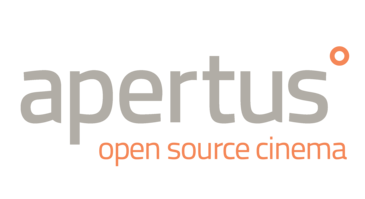
\includegraphics[width=8cm]{apertus_logo.png}}
\date{\vfill\today}

\begin{document} 
\fontfamily{qag}\selectfont
\maketitle 
\newpage
\tableofcontents
\newpage

\section{Introduction}
The aim of this task (T729) was to make a Linux kernel driver to program/debug
MachXO2 FPGAs (used as routing fabrics) in AXIOM Beta main board. This is a
report of my progress in
the first phase of GSoC 2020.\newline
Two main goals of this project are:
\begin{itemize}
\item To implement an "upload`` interface to program MachXO2
\item To implement a debug interface for OpenOCD
\end{itemize}

\section{Progress}
My milestone for the first phase (as I mentioned in my proposal) was to make a 
kernel driver with a working upload interface.
I managed to achieve this milestone in time (with a lot of help from my mentor). 
The driver can take a compressed bitstream 
(produced by Lattice Diamond tools) and upload it into MachXO2's SRAM. To
achieve this with ease, the driver integrates with Linux FPGA Framework which
provides a basic API and necessary sysfs entries. Two more sysfs entries where
added: (i) idcode: to read out 32-bit idcode from MachXO2, and (ii) rf\_status:
to read out 32-bit status register from MachXO2. Many other extra attributes 
that we need can be easily added here.\newline\newline
As of now the uploading takes about a
second, but can be optimized further. Selecting one of the two
MachXO2s (or PIC16s) as well as configuring the JTAG out ports in PIC16s is
currently taken care of by some python scripts. In future the driver will not
need these python scripts to operate.

\newpage

\section{Phase Timeline}
In the community bonding period I spent most of my time:
\begin{itemize}
\item Reading about the I2C subsystem in Linux Kernel 
\item Getting familiar and setting up my environment in the remote Betas 
\item Building my own kernel and setting up the Beta's boot options
\item Getting a basic driver up and running that recognizes the setup 
\end{itemize}

\paragraph{In this phase:}
\begin{itemize}
\item \emph{Week 1:} 
	\begin{itemize}
	\item Made the driver claim PIC addresses (0x40-0x4f) for use
	\item Studied the AXIOM Beta python scripts
	\item Added a sysfs interface and ability to read out idcode 
	\end{itemize}
\item \emph{Week 2:} 
	\begin{itemize}
	\item Read about and integrated FPGA Manager Framework with the driver 
	\item Moved all sysfs entries to FPGA Manager's sysfs interface 
	\item Added sysfs entry to read status register 
	\end{itemize}
\item \emph{Week 3 \& 4:} 
	\begin{itemize}
	\item Studied the python scripts to understand upload process
	\item Filled in API functions from FPGA Manager to upload a firmware image
	\item Setup Lattice Diamond tools and built my own image for testing
	\item Debugged the upload interface
	\item Finalized the Code
	\end{itemize}
\end{itemize}

\newpage

\section{Challenges Faced}
Most challenges I faced where about reading and understanding how things
worked and how to implement certain things in kernel driver. Understanding the
programming of PIC16, the I2C and JTAG protocols, reading documentation of
MachXO2, the Linux I2C subsystem, sysfs interface, the FPGA manager framework
and so on. Biggest challenge which I faced in the end was to get the upload
interface to actually work. Most of it was trial and error as documentation was
sparse. There were issues with hardware/python scripts, as well as
misconceptions, which made me try and change a lot of things and still get
nowhere. Even after I tried to imitate the python scripts almost exactly it
still wasn't working. Herbert, my mentor, helped me a lot in this regard. He
helped me figure out what the problem was. That we needed to upload a compressed
bitstream produced by Lattice Diamond tools instead of full binary image. After
more trial and error of testing it finally worked.

\section{Modified Timeline}
The major task in the coming two phases will be to figure out and implement a
debugging interface for OpenOCD. For this I would need to study the OpenOCD
\emph{adapters}, and maybe implement one if any of the pre existing adapters
do not suit our needs. Once the debugging interface is in place, OpenOCD can
then take care of all debugging operations and even "flashing`` the routing
fabrics.

\paragraph{In the upcoming phase:}
\begin{itemize}
\item \emph{Week 1}:
	\begin{itemize}
	\item Optimize the uploading further
	\item Add a sysfs entry to read out checksum/hash of the currently
		flashed image
	\item Add a sysfs entry to read out interpretation of status register
		bits
	\item Add the module upstream (axiom-firmware)
	\item Figure out a way to select between the two MachXO2s and configure
		the PIC16's JTAG ports from within the driver
	\end{itemize}
\item \emph{Week 2}:
	\begin{itemize}
	\item Understand OpenOCD and its internals
	\item Study and figure out how to interface OpenOCD and start
		implementing
	\end{itemize}
\item \emph{Week 3 \& 4}: 
	\begin{itemize}
	\item Add support for at least a few of the debug functionalities by the
		end of this phase
	\end{itemize}
\end{itemize}

\section{In Conclusion...}
I have learned tonnes about hardware, bus protocols, FPGAs, Linux Kernel and
many other things in just these few months with {apertus\textdegree}.
I was frustrated at times but still my interest in the project only grew. I have
really started thinking about open source hardware and its growing importance in
a way that I did not before,
and also how people here in {apertus\textdegree}
are passionately working to make it all
happen.

\end{document}
